%% LyX 2.1.4 created this file.  For more info, see http://www.lyx.org/.
%% Do not edit unless you really know what you are doing.
\documentclass[11pt,czech,american]{book}
\usepackage[T1]{fontenc}
\usepackage[utf8]{inputenc}
\usepackage[a4paper]{geometry}
\geometry{verbose,tmargin=4cm,bmargin=3cm,lmargin=3cm,rmargin=2cm,headheight=0.8cm,headsep=1cm,footskip=0.5cm}
\pagestyle{headings}
\setcounter{secnumdepth}{3}
\usepackage{url}
\usepackage{amsmath}
\usepackage{amsthm}
\usepackage{amssymb}
\usepackage{graphicx}
\usepackage{setspace}
\usepackage[final]{pdfpages}
\usepackage{natbib}
\usepackage{mathrsfs}
\usepackage{algorithm}
\usepackage{algorithmicx}
\usepackage[noend]{algpseudocode}
\usepackage{caption}

\makeatletter
%%%%%%%%%%%%%%%%%%%%%%%%%%%%%% Textclass specific LaTeX commands.
\newenvironment{lyxlist}[1]
{\begin{list}{}
{\settowidth{\labelwidth}{#1}
 \setlength{\leftmargin}{\labelwidth}
 \addtolength{\leftmargin}{\labelsep}
 \renewcommand{\makelabel}[1]{##1\hfil}}}
{\end{list}}

%%%%%%%%%%%%%%%%%%%%%%%%%%%%%% User specified LaTeX commands.
%% Font setup: please leave the LyX font settings all set to 'default'
%% if you want to use any of these packages:

%% Use Times New Roman font for text and Belleek font for math
%% Please make sure that the 'esint' package is turned off in the
%% 'Math options' page.
\usepackage[varg]{txfonts}

%% Use Utopia text with Fourier-GUTenberg math
%\usepackage{fourier}

%% Bitstream Charter text with Math Design math
%\usepackage[charter]{mathdesign}

%%---------------------------------------------------------------------

%% Make the multiline figure/table captions indent so that the second
%% line "hangs" right below the first one.
%\usepackage[format=hang]{caption}

%% Indent even the first paragraph in each section
\usepackage{indentfirst}

%%---------------------------------------------------------------------

%% Disable page numbers in the TOC. LOF, LOT (TOC automatically
%% adds \thispagestyle{chapter} if not overriden
%\addtocontents{toc}{\protect\thispagestyle{empty}}
%\addtocontents{lof}{\protect\thispagestyle{empty}}
%\addtocontents{lot}{\protect\thispagestyle{empty}}

%% Shifts the top line of the TOC (not the title) 1cm upwards 
%% so that the whole TOC fits on 1 page. Additional page size
%% adjustment is performed at the point where the TOC
%% is inserted.
%\addtocontents{toc}{\protect\vspace{-1cm}}

%%---------------------------------------------------------------------

% completely avoid orphans (first lines of a new paragraph on the bottom of a page)
\clubpenalty=9500

% completely avoid widows (last lines of paragraph on a new page)
\widowpenalty=9500

% disable hyphenation of acronyms
\hyphenation{CDFA HARDI HiPPIES IKEM InterTrack MEGIDDO MIMD MPFA DICOM ASCLEPIOS MedInria}

%%---------------------------------------------------------------------

%% Print out all vectors in bold type instead of printing an arrow above them
\renewcommand{\vec}[1]{\boldsymbol{#1}}

% Replace standard \cite by the parenthetical variant \citep
%\renewcommand{\cite}{\citep}

\makeatother

\usepackage{babel}
\begin{document}
\def\documentdate{July 7, 2017}

\newtheorem{definition}{Definition}[chapter]
\newtheorem{note}{Note}[chapter]
\newtheorem{example}{Example} 

\newtheorem{theorem}{Theorem}

\captionsetup[figure]{labelfont={bf},labelformat={default},labelsep=period,name={Fig.}}


\def\documentdate{\today}

\pagestyle{empty}
{\centering

\noindent %
\begin{minipage}[c]{3cm}%
\noindent \begin{center}

\includegraphics[width=3cm,height=3cm,keepaspectratio]{Images/TITLE/cvut}
\par\end{center}%
\end{minipage}%
\begin{minipage}[c]{0.6\linewidth}%
\begin{center}
\textsc{\large{}Czech Technical University in Prague}{\large{}}\\
{\large{}Faculty of Nuclear Sciences and Physical Engineering}
\par\end{center}%
\end{minipage}%
\begin{minipage}[c]{3cm}%
\noindent \begin{center}

\includegraphics[width=3cm,height=3cm,keepaspectratio]{Images/TITLE/fjfi}
\par\end{center}%
\end{minipage}

\vspace{3cm}


\textbf{\huge{}Real Options Valuation: A Dynamic Programming Approach}{\huge \par}

\vspace{1cm}


\selectlanguage{czech}%
\textbf{\huge{}Oceňování projektů metodou reálných opcí z pohledu dynamického progamování}{\huge \par}

\selectlanguage{american}%
\vspace{2cm}


{\large{}Master's Thesis}{\large \par}

}

\vfill{}

\begin{lyxlist}{MMMMMMMMM}
\begin{singlespace}
\item [{Author:}] \textbf{Filip Rolenec}
\item [{Supervisor:}] \textbf{Ing. Rudolf Kulhavý, DrSc.}
\end{singlespace}

\item [{Language~advisor:}] \textbf{Ing. Rudolf Kulhavý, DrSc.} 
\begin{singlespace}
\item [{Academic~year:}] 2020/2021\end{singlespace}

\end{lyxlist}
\newpage{}

~\newpage{}

~

\vfill{}


\begin{center}
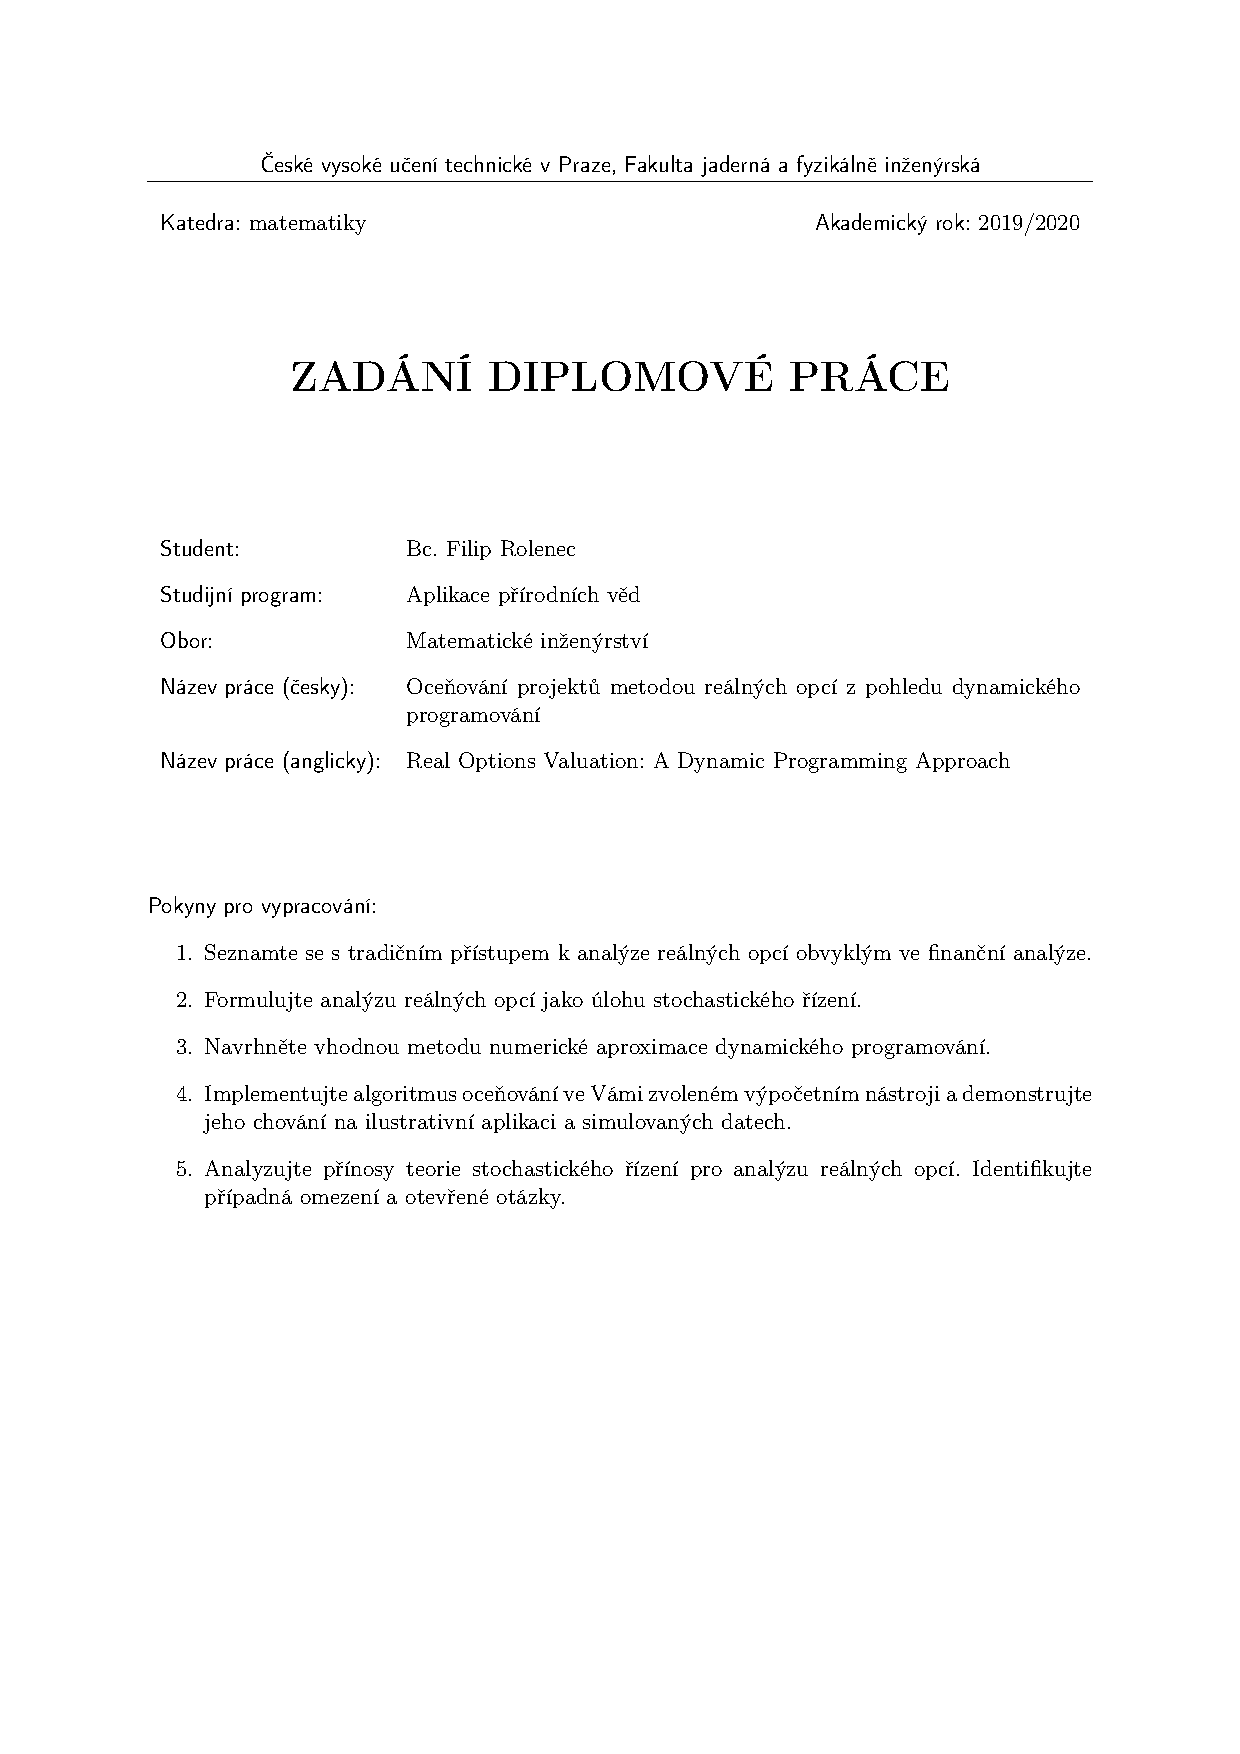
\includepdf[pages={1}]{Images/zadaniMT.pdf}


\par\end{center}

\vfill{}


~\newpage{}

~

\vfill{}


\begin{center}
\includepdf[pages={2}]{Images/zadaniMT.pdf}
\par\end{center}

\vfill{}


~\newpage{}

\noindent \emph{\Large{}Acknowledgment:}{\Large \par}

\noindent I would like to thank my supervisor Ing. Rudolf Kulhavý, DrSc. for his professional guidance and all the advice given while creating this thesis. 

\vfill

\noindent \emph{\Large{}Author's declaration:}{\Large \par}

\noindent I declare that this Master's thesis is entirely
my own work and I have listed all the used sources in the bibliography.

\bigskip{}


\noindent Prague, \documentdate\hfill{}Filip Rolenec

\vspace{2cm}


\newpage{}

~\newpage{}

\selectlanguage{czech}%
\begin{onehalfspace}
\noindent \emph{Název práce:}

\noindent \textbf{Oceňování projektů metodou reálných opcí z pohledu dynamického progamování}
\end{onehalfspace}

\bigskip{}


\noindent \emph{Autor:} Filip Rolenec

\bigskip{}


\noindent \emph{Obor:} Matematické inženýrství 


\bigskip{}


\noindent \emph{Druh práce:} Diplomová práce

\bigskip{}


\noindent \emph{Vedoucí práce:} Ing. Rudolf Kulhavý, DrSc.


\bigskip{}


\noindent \emph{Abstrakt:} Oceňování převážné většiny investičních příležitostí se dnes stále určuje metodou \textit{diskontovaných peněžních toků} (DCF) \ref{}. DCF metoda je přímočará a pro jednoduché projekty dává velmi přesné výsledky. Složitější projekty, které pro tuto práci definujme jako projekty s vysokou mírou vnitřní neurčitosti a existencí manažerských rozhodnutí značně ovlivňujících strukturu projektu (reálné opce), jsou dnes oceňovány metodou \textit{real option analysis} (ROA). Metoda ROA přiznává hodnotu možnostem změny projektového plánu, v důsledku čehož je ohodnocení ROA vyšší než DCF. 

Tato práce má za cíl interpretovat řízení projektů a s ním související ocenění, jako řízení stochastického systému. Rozsáhlá teorie stochastického řízení \ref{}, \ref{}, \ref{}, dovoluje vybudovat novou teorii oceňování postavenou na základech ROA, která mimo jiné řeší omezení ROA na pouze jediný zdroj neurčitosti - například cenu těžených minerálů na trhu \cite{}. 

Nový originální přístup k oceňování projektů, který kombinuje dosavadní dosažené znalosti v ekonomické teorii (ROA) a teorii stochastického řízení systémů (SDT) je obecně definován v první části práce a prakticky otestován simulacemi na třídě problémů z oblasti  <Area of study>. 

Simulace ukazují, že kromě lepší interpretovatelnosti modelu a možnosti vložení subjektivních pravděpodobností je ocenění metodou ... přesnější o ... \%. Výsledky vyjadřují naději na zvýšenou adopci metody ... v praxi. 


\bigskip{}


\noindent \emph{Klíčová slova:}   Analýza reálných opcí, Diskontované peněžní toky, Oceňování projektů, Stochastické řízení, Těžební průmysl



\selectlanguage{american}%
\vfill{}
~

\begin{onehalfspace}
\noindent \emph{Title:}

\noindent \textbf{Real Options Valuation: A Dynamic Programming Approach}
\end{onehalfspace}

\bigskip{}


\noindent \emph{Author:} Filip Rolenec

\bigskip{}


\noindent \emph{Abstract:} The valuation of investment opportunities (projects) is nowadays still predominantly computed by the\textit{ discounted cash flow } (DCF) method \ref{}. DCF is straightforward and gives solid results for simple projects. For more complicated projects, which are in this thesis defined as projects with substantial degree of inner uncertainty and with an existence of ability to change the course of the project by direct managerial actions, the \textit{real option analysis} (ROA) is now being used. ROA recognizes the value in the possibility of projects' plan change, which usually results in loss limitation, increasing the project's overall expected value. 

This thesis aims to interpret project execution and its valuation as a problem of stochastic decision control. The extensive stochastic decision control theory (SDT) allows, based on ROA,  to design new valuation theory, that for example solves the limitation of ROA on only one source of uncertainty - such as the volatile price of the mined materials on the market. 

The new and original approach to project valuation, that combines both the economical theory (ROA) and the stochastic control theory is defined in the first part of the thesis and then tested by simulations on a class of valuation problems - valuation of projects in <Industry>.

Simulations show that in addition to better model's interpretability and a possibility to include a personal probability distributions, the valuation by <method> is <percentage> more precise than best current strategies. The results hint a possible increase in adoption of this method in practice. 

\bigskip{}


\noindent \emph{Keywords:} Discounted cash flow, Mining industry, Project valuation,  Real option analysis, Stochastic decision control

\newpage{}

~\newpage{}

\pagestyle{plain}

\tableofcontents{}

\newpage{}


\chapter{Introduction}

The current state of capital investment valuation techniques is a mess. Majority of investors still rely on the standard Net Present Value (NPV) technique or its slight generalizations in form of optimal/average/bad scenarios, risk adjusted discount rate (RADR) hurdles (usually set to an arbitrary percentage), internal rate of return (IRR) metric (which is essentially the same as RADR hurdles) and other metrics like,... ROIC, ENPV. 

All the listed generalizations try to cope with one of two main problems of NPV, which is inability to incorporate uncertainty (ENPV, scenario approach) or intra-investment comparison (IRR(?), ROIC). 

None of these valuation techniques acknowledges the managerial ability to take action and improve the course of an investment. ENPV can be interpreted is such way but that is abusing of its notation. 

The decision tree analysis (DTA) is the simplest approach for valuing an investment with acknowledging decision nodes as an inherit trait of an investment process. It should not be a surprise that being able to make a decision through the lifetime of an investment has value. Also, it is quite clear that the more uncertain the investment and its parts are, the more valuable the ability to act is. To value an ability to make a decision and change the path which the investment follows is not a complicated task. All it takes is to compare a value of a project with that ability and without it (both with DTA), and declare that the value of such "decision option" is the difference between the two. 

Many authors from the financial world \footnote{See \textit{this} and \textit{that}} use the term real option valuation when talking about this difference between DTA trees with or without some branches that represent the ability to make a decision and act upon it. I think that is rather unfortunate, since the terminology clashes with the real option valuation, which this thesis is about. 

The true real option analysis (ROA) is about being able to value investment options in the same way financial options are valued. The Black-Scholes-Merton option pricing model that is widely used in financial world is an exceptionally elegant valuation tool. All that it needs to know about financial option to valuate it is four parameters - the strike price and expiration date of an option itself, the volatility and current price of the underlying asset upon which the option is written. \footnote{probably some more assumptions}. This Nobel-Prize winning elegance led mathematical and financial experts to try to interpret investment decision making in terms of "real options", that can be valued in the same way the financial options are, by the BSM model. 

The attempts to interpret each of four important parameters of a financial option in terms of investment parameters are successful for simple cases (Dealership in BERK), however they fail for more complex ones. The ability to use real option valuation technique depends heavily on the ability to find a relevant company, stock or other publicly traded proxy variable to the examined investment. One finds plausible to construct a replicating portfolio for an investment in oil mining facility or a food production line, however this assumption is hard to believe for highly innovative products in new fields, such as software development or R\&D investments. 

The ROA valuation approach in investment decision making has cyclical nature. The first wave of the real ROA approach can be traced to ... who presented his ideas shortly after the initial publication about financial option pricing \cite{BlaSch:73}. Next wave comes with ... and finally the most recent publications trying to make practical use of real option analysis are \cite{} and \cite{}. 

Nearly all publications of real options published in the last <number> years talk about small penetrability of this approach to the actual usage by managers in large and small investment companies. The stated reasons are always the same,
\begin{itemize}
\item Vollert says that its complexity, but that is because he uses stochastic models, Ito lemma and computes PDEs, all the time. That has nothing to do with replicating portfolios and BSM model. 
\item Mr. Kulhavy says that the problem is in finding the replicating portfolio and even if you find it you have to persuade the manager to see it too. 
\item <Problem with adoption> 
\item <Another problem with adoption>
\end{itemize}


I believe that the current usage of ROA by investors makes sense. The actual ROA approach is based on finding a replicating portfolio that behaves in the same way as the investment. If a manager beliefs that he has found a replicating portfolio, then it does not make sense for him to value the project differently than the replicating portfolio. However, there is still the issue of finding such replicating portfolio. 

The usage of ROA in sense of different DTA trees is well posed. The ability to hold production in refinery in times of large oil prices can surely increase its value. In this sense the ROA has the biggest impact on the valuation in investments that are highly uncertain and in which there are actions that can alter the course of future cash flow. This also means that in the opposite case, when there is high degree of certainty about the execution and cash flow of the project, or if there are no actions to be taken, the ROA does not create additional value. 

The power of classic ROA is to seemly eliminate the probabilistic nature from the picture. This can be done by the power of all-wise market, that forbids the existence of arbitrage. If a tradeable  \footnote{This is a valid word, Cambridge dictionary say so... }replicating portfolio is found, then I should not care if I make my investment or if I use the money to buy the replicating portfolio. 

For the mathematicians from the field of stochastic decision making the problem of valuation is just another decision making under uncertainty. Define state  and action space, define rewards (free cash flow) in each epoch and get prior probability density as expected transition probability from one state to another upon undertaking certain action.

The difference between the SDT and ROA is that the former relies on the prior density functions, that are the core of Bayesian statistic, while the latter, coming from economics, relies on the power of the market and managers ability to find a replicating portfolio. 

In this thesis the state-of-the art theories of ROA valuation and SDT are presented. Their strengths and weaknesses are discussed and a hybrid approach from the cherry-picked parts of the corresponding theories is presented. 

The power of the new theory is shown on a class of problems called ... The current literature copes with them in much simpler way and their assumptions are much larger. My \footnote{Or the presented approach, should I avoid pronouns in the text? } approach also potentiates adoption in practical usage, as it puts the decision making manager in charge. The manager decides how to create the prior distributions, he is the one who needs to determine all the possible actions and scenarios that can happen. The algorithm that is presented in this thesis can and should be used in real world as a managerial tool to maximize the profits of divisions or companies as a whole. 


The goal to maximize wealth in financial world is approached in a really narrow matter. Money represents value, which in models decreases in time by a percentage given by some authority, most of the time central banks. In respected financial publications \cite{BerDeM:09}, \cite{} or \cite{}, there is no notion of utility. It seems like for financial institutions, it does not matter to get 1M in cash now or to gamble for 2M in a fair coin flip. On the other hand, in SDT,  the concept of utility is taken very seriously. Most of the people would prefer even such a small amount as 200k against a fair gamble between 0 and 2M. This is due to the concave utility function people tend to have when very high amounts are discussed. 

Maximization of wealth either in the sense of investment company or individual is natural. Almost everybody would agree that to have more wealth is better than have less. Better investment decisions mean higher accumulation of wealth, which together with assumption of free market result in an increase of utility of each participant in the economy \footnote{Find that reference... Duke university lectures... }. In other words, when a company makes higher profits it should mean that the part of the population that participated in the wealth creation should be happier. 



%\addcontentsline{toc}{chapter}{Introduction}



%\addcontentsline{toc}{chapter}{Preliminaries}

\pagestyle{headings}

\chapter{Preliminaries}

To understand the main message of this thesis it is important to present several key financial and mathematical concepts. Two main concepts that will be examined in this thesis are Real Option analysis (ROA) and stochastic decision theory (SDT).

\section{Classic valuation techniques}
For clarity of the further research lets define the basic valuation techniques. Even though, or maybe exactly because, they are simple, they are widely used in investment companies today. All techniques are based on an idea of cash flow per sample period, where cash flow is clear profit, already adjusted for expenditures, taxes, and all other mathematically distracting aspects of accounting. 

\subsection{Net Present Value} 
This metric is mentioned in almost all publications about valuation techniques. It is simple and it takes into account time value of money. The classic definition of NPV is: 

\begin{equation}
	NPV = \sum_{t \in \mathbf{T}} \frac{C_t}{r^t}, 
\end{equation}
where $\mathbf{T}$ is set of time periods in which free cash flow $C_t$ is obtained. Discounting factor $r^t$ expresses the time value of money and it is expected to be positive. In the light of recent events in advanced economies like that of Japan, Switzerland and Germany, the positivity of this variable is not a clear cut. Unprecedented moves of the central banks of these countries to boost the economy by negative interest rates might cause a problems in NPV valuation, since many examples \cite{},... rely on the fact that an infinite sum of constant cash flows discounted by any factor $r>1$ converges. 

However that is not the concern of this publication and we will assume that $r>1$.

The NPV valuation technique is simple to use, assuming we know the discount rate, which is constant through the lifetime of the investment, and free cash flows, that are expected to be certain. 

The problem with this valuation arises if we acknowledge that the discount rate, or cash flows, or both can be uncertain. Two possible valuation techniques emerge from this uncertainty. First there is the simple scenario approach, in which the valuation committee decides cash flows and/or interest rate evolution scenarios as bad, neutral and good. This is unfortunately effectively the pinacle of valuation techniques in some investment companies. 

Second type concerned with uncertainty is ENPV valuation. 

\subsection{ENPV valuation}
The simplest approach how to handle uncertainty is to use expected values of the random variables that occur in the classic NPV equation. Now it is accepted that cash flow $C_t$ and also discount rate is a random variable. In both cases it is expected that the distribution of these variables is known. The ENPV valuation is then: 
\begin{equation}
	ENPV = \sum_{t \in \mathbf{T}} E[\frac{C_t}{r^t}] = \sum_{t \in \mathbf{T}} \frac{p(C_t)C_t}{p(r_t)r_t^t}. 
\end{equation}


\subsection{Comparing investments}
There could be some part where metrics that are used to favor one investment over the other here. Comparing NPVs only seems not a good idea, but for example ROIC seems much better and the simplest strategy I would use for investment decision making. 

Also comparing IRR and other statistics seems like a magic, maybe because in the end the decision is only backed by these numbers, but the feeling manager has is what the decision is based upon. 


\subsection{Other frequently used valuation techniques} 
Probably not needed, thus it should not be here. Just an idea. IRR, EVA, EPS,... 


\subsection{Decision tree analysis}
The decision tree analysis, which was introduced in... is the first valuation technique that acknowledges the importance of further management of investments. In some sense it is equivalent to a NPV with a number of scenarios equal to number of leaves in the decision tree representing an investment. 

Decision tree analysis is based on creation of a decision tree, with three type of nodes. Decision nodes serve as a representation of an opportunity to take action by the decision maker, whereas \textit{probability} nodes serve as a representation of an uncertain event that cannot be modified. 

As can be seen in many many articles the added value of acknowledging the possibility to act upon the existing investment can be crucial. In more dynamic environments this value increases, since there is generally a bigger change between cash flows of different actions. 

It bewilders me, from the terminology perspective, how some authors interpret a difference between two different DTA trees as an "Real option". However from the linguistic point of view that makes sense. A new branch in a decision three is literally a new option (real option) to act upon resolution of uncertainties in an investment. 

\section{Real option analysis}
The idea to analyze investment opportunities and their parts as options that are available to a decision maker came right after a widely recognized valuation technique of financial options was adopted. This technique is of course the Nobel-prize wining Black-Scholes-Merton model, first published in \cite{BlaSch:73} which allows to value financial option with only small requirements and a widely accepted assumptions. 

Based on this valuation model, group led by ... came up with the idea to adopt this type of thinking into real project investment decision. The similarities between simple project investments and financial options are clear, but for more complicated projects, this interpretation starts to be less and less viable. Further discussion is left to next chapters. 

\subsection{Financial options}
The rise of the derivative market of futures and options comes from the idea of insurance against the fluctuation of commodity prices on the market. To secure against the unwanted shifts in the price of a commodity viable for running a business certainly has value for the participants of the economy. The question long time (?) was how large this value is. 

A financial option is an ability to buy or sell an asset for a given price in some time in the future. A financial option can be also defined by its two properties, price for which shares can be bought (in case of call option) or sold (put option) - strike price, and the time at which the option can be realized - time to maturity. Furthermore there are two types of options european and american, which have the ability to execute the option earlier than the maturity time. Because it was proved that executing an option earlier than in the time of maturity \cite{}, it does not matter which options are we going to talk about.  

<Also talking only about calls since puts are not important in real options> 

An example of a financial option from current market can be the option to buy Amazon stock currently valued 2286 for 3000 USD in 17-7-2020. This option has a price tag of 11 USD at the time of writing. 

Option speculation is interesting because it allows the investor large profits if the markets move in the right direction. For example if the price of Amazon stock from the previous example will be 3110 USD, then an investor into those type of options can count with a 1000\% profit. 

The question now is, where did the price tag for an option came from. A elegant answer lies in the Black-Scholes model for option pricing. 


\subsection{Black-Scholes Merton model}
Only four parameters and one assumption is needed to determine a value of an option according to BSM model for option pricing. Assume that the market is complete, and thus the law of one price holds \cite{}. Then to value a option you need to know only its time to maturity, its strike price, the current price of the underlying stock and its volatility as follows \cite{BerDeM:09}: 
\begin{equation}
	C = SN(d_1) - PV(K)N(d_2), 
   \label{BSMModelEq}
\end{equation}
where $S$ is the strike price, $PV(K)$ is a price of a bond paying K on the expiration day of the option and $N(d)$ is a cumulative normal distribution, probability that a normally distributed variable is less than $d$. Value of $d_1$ and $d_2$ is then defined as: 
\begin{equation}
	d_1 = \frac{ln(S/PV(K))}{\sigma \sqrt{T}}+\frac{\sigma \sqrt{T}}{2}
	d_2 = d_1 - \sigma \sqrt{T}
\end{equation}


The dependency of the price of an option is positive in case of volatility and time to maturity Increasing these parameters leads to a higher option price. On the contrary the rise in current stock price or strike price of the options lowers the value of an option. 


\subsection{Real options}
<Difference in DTAs, analogy for financial options, or CAPM model?>




\section{Statistical decision theory}
The second pillar upon which this thesis stands is the statistical decision theory. An area of applied mathematics with broad history. The class of problems that can be solved by this approach is very wide and greatly standardized. 

The STDs main focus is to determine the optimal decision to act upon in dynamic and uncertain environment. A classical structure of a decision making problem is: ... 

In SDT the uncertainty is modeled by the transition probability function which is either assumed to be known, or it is being estimated by either classical statistic methods or Bayesian methods. 

The optimal decision strategy (sequence of actions) is the one that gives the maximal cumulative reward. This maximization can be total (in finite or discounted cases) or per period. We will focus on the total cumulative reward in finite processes (?)

To compute value function in all decision nodes of the grid of statistical decision theory a smart idea of backward induction, called dynamic programming is used. The narrative that a sequence of actions is optimal if and only if the last action of the sequence is clear, but powerful when used in this context. Instead of going through
 <something like $S^{A^B}$ possible 
paths and computing expected cumulative reward for all of them, one can optimize his actions from the horizon, lowering the number of computations needed significantly to an order of <something like $S^A*N$ ...>. For example if the scale of the problem is ... the change is from $10^100$ to $10^20$. 

To obtain a value function in each decision node of the stochastic decision process a Bellman equation is used. 

\begin{equation}
	TODO -BELLMAN EQ
		\label{BellmanEq}
\end{equation}

When valuing an investment both statistical approaches to estimation are used, but in different cases. The statistical theory allows to estimate parameters when a lot of data is present (for example to determine a volatility of a stock). On the other hand, when the data is scarce and the decision making is undertaken by an expert, the Bayesian theory enables to import his subjective idea into the process. 

\subsection{Bayesian statistics}
<Bayesian statics allow to include subjective opinion of the uncertainty> 
<Bayesian statistics are based on randomization of a parameter>
<There is a model for the data in the same way that in classical statistics>
<Not even classical statistics is objective, since you always have to choose a model> 
<Bayes equation, updating on data, certainty equivalence,...> 

\subsection{Utility}
When rewards are not valued linearly by the decision maker the concept of utility comes in. One of the simplest examples to demonstrate the usage of utility is given by \cite{BacChi:19}. Imagine you are given a choice, either get 500\$ right away or gamble for 1000 \$ in a fair coin toss. A rational decision maker driven only by the expected value given should be indifferent to these choices, but the majority of people tend to take the certain option \cite{}. The decision making is clearer as the amount of money rises, there is a little difference for an average human to obtain 10M and 20M, the change in his life will be almost the same with both results. However one is certain and the other is not. 

Another interesting example of utility is the St. Petersburg paradox <find reference> where rational decision maker should be willing to pay unlimited amount of money to be able to play the game, but people are seldom willing to pay more than ... 

There is also an interesting asymmetry between incurring a loss and getting a profit. This can be seen from picture ... \cite{BacChi:19}. 

Each person has their own utility function with respect to money and it can be sketched essentially by a questionaire. More questions mean more precision, and it also keeps your answers coherent.  


\section{Approximate dynamic programming}
<Why it exists and what are the types?>
Actual application of classic dynamic programming 

\chapter{Real option analysis in terminology of stochastic decision control}
The similarity of ROA and SDT is clear (?). 

MAIN PART OF THE THESIS 




\chapter{Application of the cheery-picked valuation technique. }
The class of .... valuation problems is ideal for demonstration of the usability of the newly developed valuation technique. Due to the inherit uncertainty in this field and many actions that can be undertaken, the additional value  assigned to the investment opportunity can be significant. 

We start with a rigorous mathematical definition of this class of valuation techniques in terms of SDT. Then we pick one example and promptly show that the number of possible states is exponential with respect to... Approximate dynamic programming techniques like Q-learning or SARSA were developed in order to solve exactly these types of problems. Due to their strengths and only a minor flaws their usage is justified. 


 \section{Approximate dynamic programming}
<Proposal of a fitting method to the class of problems defined above> 

\section{Valuation example}
 
 \subsection{NPV valuation }
 
 \subsection{DTA valuation}
 
 \subsection{Classic ROA valuation}
 
 \subsection{New approach}
 


\chapter{Discussion}
The new approach is better because it solves the current problems with ... Also the applicability of the new approach is in my opinion broader since it can address multiple sources of uncertainty. Furthermore the power of the decision making process is kept in the hands of the decision maker through creation of prior distributions. The manager is guided through the world of utility functions and priors, which both can be created from a set of simple questions about gambles and beliefs of the manager. The creation and usage of the utility and prior density functions are fool-proof in a sense of mathematical coherence. 




\chapter{Conclusions}
In my master's thesis I have rigorously compared the state-of-the-art valuation techniques used in present investment companies. I have shown the advantages and disadvantages of real option analysis  and stochastic decision theory. The combination of these, which I call ...,  yields a new view on the world of risky investments that empowers the decision maker and thus allows for better adoption in the rigid environment of investing. 







\chapter{Bachelor's thesis parts that could be useful for TeX styling}




\section{Discrete Markov decisions processes}\label{DMDPSection}
A lot of real life decision tasks can be approximately described by the mathematical framework called discrete Markov decision processes (MDPs), Fig. XY. The definition of this mathematical framework is crucial for this work, as it is the basis upon which the theory of policy optimisation is built. 

\begin{definition}
	Discrete Markov Decision Process $\mathcal{M}$ is defined as ordered set of five elements $(\textbf{T},\textbf{S},\textbf{A},P,R) $, where:
	\begin{itemize}
		\item \textbf{T} stands for a discrete, finite set of decision epochs; $\textbf{T}=\{0,1,2,...,|\mathbf{T}|\}$, where\footnote{Because the number of time epochs $|\mathbf{T}|$ is used frequently, the notation $|\mathbf{T}|=N$ is used.} $|\mathbf{T}| \in \mathbb{N}$
		
		The state in time epoch $t=0$ is known and it is denoted $s_0$.
	\end{itemize} 
	
\end{definition}\label{DMDP}


\begin{definition}\label{ValueF} 
	Let $\mathcal{M}=(\textbf{T},\textbf{S},\textbf{A},P,R)$ be a MDP and $\pi_t \in \mathbf{\mathbf{\Pi_t}}$ a policy, then \textbf{value functions} of $\mathcal{M}$, $\varphi_{t}^{\pi_t}: \mathbf{S}\rightarrow \mathbb{R}$ are defined $\forall \pi_t \in \mathbf{\Pi_t}$, $\forall t \in \mathbf{T}\setminus \{N\}$ as:
	\begin{equation}
	\varphi_{t}^{\pi_t}(s)=E\bigg[\sum_{\tau > t, \tau \in \mathbf{T}}R(s_\tau,a_{\tau-1},s_{\tau-1})\big|s_t=s\bigg], 	
	\end{equation}
	
\end{definition}


\begin{theorem}\label{DynProgTheo}
	Let $\mathcal{M}=(\textbf{T},\textbf{S},\textbf{A},P,R)$ be a MDP, then the optimal value function $\varphi_t^{o}(s)=\max_{\pi_t \in \mathbf{\Pi_{t}}}\varphi_t^{\pi_t}$ can be computed recursively $\forall t \in \mathbf{T}\setminus\{N\}$ through the equation:
	
	\begin{equation}
	\varphi_t^{o}(s)=\max_{a_t \in \mathbf{A}} E\bigg[R(s_{t+1},a,s) + \varphi_{t+1}^{o}(s_{t+1})|a_t,s\bigg],
	\label{DynProgEq}
	\end{equation}
	considering that $\varphi_{N}^{o}=0$ as Definition \ref{ValueF} implies. Furthermore the optimal policy $\pi_{t}^{o}$, as the argument of maxima, is concentrated on maximising arguments in Equation (\ref{DynProgEq}). 
	
\end{theorem}

\begin{proof}
	This theorem will be proven via a finite backward mathematical induction.
	
	At first, let us take an action $a^{o}_{N-1}$ in the time epoch $N-1$ defined as:
	\begin{equation}
	a^{o}_{N-1}(s) = \mathrm{Arg}\max_{a\in\mathbf{A}} E[R(s_{N},a,s)|a,s].
	\end{equation}
	By the definition of maxima the inequality
	
\end{proof}


We can now describe the dynamic programming algorithm in detail.

\begin{algorithm}
	\caption{Finding the optimal policy for a \textit{single system} MDP with known $P$}\label{alg:SingleKnown}
	\begin{algorithmic}[1]
		\Require{$\mathcal{M}=(\textbf{T},\textbf{S},\textbf{A},P,R)$}
		\State$ \varphi_N^{o}(s) \gets 0$, $\forall s \in \mathbf{S} $ \Comment{Based on Definition \ref{ValueF}.}
		\State $t \gets N$ 
		\While{$t\ne 0$}
		\For{ each $s \in \{1,2,...,|\mathbf{S}|\}$}
		\State $\varphi_{t-1}^{o}(s) \gets Equation$ $(\ref{DynProgEq})$ \Comment{With known $P$ and $\varphi_{t}^{o}$}
		\EndFor
		\State $t \gets t-1$
		\EndWhile
		\State $\pi_{0}^{o}(s) \gets argmax$ $\varphi_0^{o}(s)$ $ \forall s\in \mathbf{S}$, \Comment{Deriving the optimal policy}
		\State	\Return{$\pi_{0}^{o}$}
	\end{algorithmic}
\end{algorithm}




\begin{example}\label{Ex:Multi}
A real life example of this MDP could be again a biased coin tossing. Imagine a game when you are sitting at the table on which there are multiple coins with generally different bias. You get one coin on certain side in your hands and you are told the rules. You get $\$$1 each time the coin lands on Heads. You can choose to change your coin for any other coin for $\$$3 and you have to place it to the side it is on the table (you have to "conserve its state"). The turn of the coin costs 5 cents and the result of the toss generally depends on the side from which the coin is tossed. You know the bias of each one coin and the question is: what is the best sequence of actions that you can perform to get as much money as possible, on average, from this $N$-round game?

It is important to mention that you are able to see the other coins "on the table" so that the position state $s^{p}$ is known in each time epoch. 
\end{example}



\paragraph{Discussion}
The main goal of this simulation is to check the quality of the experimentally derived sub-optimal policy via Algorithm \ref{alg:SingleKnown}. As we can see, the difference between the average cumulative reward of the derived policy and the expected optimal average cumulative reward is approximately $0.5\%$ in the first simulation with 500 Monte Carlo iterations and approximately $0.026 \%$ in the second simulation with 5000 iterations.  \footnote{I dont know how to fit the exceedance in here, so if it is not that important I would prefer not to talk about it.}

We can also see that in the second performed experiment made for 5 000 iterations, ten times the first case, both the variance of the distribution and the difference from the optimal value decreased. It is then assumed that this trend would continue with more iterations and that both the variance and the difference would get closer and closer to zero.

With this assumption we can say that the experimentally derived optimal policy is in fact the optimal one. \footnote{Is that a good reasoning?}




\begin{table}[H]
	\centering
	\renewcommand{\arraystretch}{2}
	
	
	\begin{tabular}[t]{|r|r |r|}
		\hline
		\multicolumn{3}{|c|}{$P(:,:,s=1)$} \\
		\hline
		$\tilde{s}$/$a$  & 1 & 2\\
		\hline
		1	& 0.4237&	0.6885\\
		\hline
		2 & 0.5763 & 0.3115 \\ 
		\hline
		
		\multicolumn{3}{c}{} \\[-0.4cm]
		\hline
		\multicolumn{3}{|c|}{$P(:,:,s=2)$} \\
		\hline
		$\tilde{s}$/$a$ & 1 & 2\\
		\hline
		1	& 0.7282&	0.8816\\
		\hline
		2 & 0.2718 & 0.1184 \\ 
		\hline
	\end{tabular}
	\hfill
	\begin{tabular}[t]{|r|r |r|}
		\hline
		\multicolumn{3}{|c|}{$R(:,:,s=1)$} \\
		\hline
		$\tilde{s}$/$a$  & 1 & 2\\
		\hline
		1	& 1.4315&	-0.0569\\
		\hline
		2 & 2.7287 & -0.3111 \\ 
		\hline
		
		\multicolumn{3}{c}{} \\[-0.4cm]
		\hline
		\multicolumn{3}{|c|}{$R(:,:,s=2)$} \\
		\hline
		$\tilde{s}$/$a$ & 1 & 2\\
		\hline
		1	& -0.1039&	2.5921\\
		\hline
		2 & 1.1251 & -0.2876 \\ 
		\hline
	\end{tabular}
	\hfill
	\begin{tabular}[t]{|r|r |r|}
		\hline
		\multicolumn{3}{|c|}{$w(:,:,s=1)$} \\
		\hline
		$\tilde{s}$/$a$  & 1 & 2\\
		\hline
		1	& 8&	5\\
		\hline
		2 & 1 & 2 \\ 
		\hline
		
		\multicolumn{3}{c}{} \\[-0.4cm]
		\hline
		\multicolumn{3}{|c|}{$w(:,:,s=2)$} \\
		\hline
		$\tilde{s}$/$a$ & 1 & 2\\
		\hline
		1	& 1&	2\\
		\hline
		2 & 9 & 1 \\ 
		\hline
	\end{tabular}
	\caption{Tables of $P$, $R$ and $w$ values for the CE approach simulation. Original 3D arrays are presented by two  "slices" which differ in the initial state $s=1$ or $s=2$. }\label{Tab:PRwValues}
\end{table}\footnote{Hope this representation is OK, and how to do the backslash $\tilde{s},a$?}


\pagestyle{plain}

\bibliographystyle{plain}

\bibliography{fr}




\end{document}
